% Hypothesis
% \begin{itemize}
%     \item Separability is important
%     \begin{itemize}
%         \item Separation sets
%         \item All positive network
%     \end{itemize}
%     \item Controlling separability enhances the network
%     \begin{itemize}
%         \item Depth
%         \item Dead units
%         \item Zero init
%         \item Moons data shattering
%     \end{itemize}
%     \item Separability works in real world
%     \begin{itemize}
%         \item Toy Cifar
%         \item SimpNet
%         \item ULMfit
%         \item Fixup
%     \end{itemize}
% \end{itemize}

\section{Experiments and Results}\label{sec:experiments}
After presenting the separability constraints, we test our formulation in an example of a \ReLU-based network (of depth $d=50$, and fixed layer width $N_k=4$), specially targeted to: 
\begin{enumerate}
    \item fail to trivial accuracy values with \ReLU and batchnorm.
    \item exhibit the highlighted issues that DNN experience: dying neurons, vanishing gradient, and to some extent exploding gradient.
    \item is manageable enough to relate to analytical results presented previously.
\end{enumerate}
Experimentation was done over two datasets: the \moons dataset (for \emph{toying}) and the \texttt{CIFAR-10} to test in a more realistic setting involving (a CNN with $5\times 5$ kernels with padding to preserve image size), using \texttt{Keras} and \texttt{TensorFlow}.
\\\\
Within the \moons dataset we sampled $100$ points ($85$ for training and $15$). As hyper-parameters, we used learning rates $\gamma \in \{0.01, 0.001, 0.0001\}$, a batch size $bs = 85$, to ensure \emph{fairness} for \SepUnit.  For testing, the loss functional $\mathcal{L}$ in equation \ref{eq:constraintLossFunctional}  was chosen to be the cross-entropy as presented in \cite{LeCun06atutorial}, introducing constraint loss parameter $\lambda = 0.01$ using $T = 2000$ epochs. 
\\\\
Due to the fact that \cifar is a much larger dataset, choosing hyper-parameters for experimentation were chosen empirically. Learning rates are \emph{smaller} than the ones used for \moons: $\gamma \in \{0.001, 0.0005, 0.0001 \}$, while extending experimentation to two batch sizes: $64$ and $128$.  Constraint trade-off parameter $\lambda$ was tuned using: $10^{-5},10^{-3}$ and $1$ values, and for the sake of speed we set the number of epochs to $T = 500$.
\\\\
In matters of \emph{initialization} two schemes were tested: the \emph{Glorot Uniform Scheme} implemented in \texttt{Keras} following (see \cite{Glorot10Initialization} for the technical details) and \emph{zero initialization} consisting in setting weights and biases to zero. 

\subsection{Results concerning Accuracy}\label{subsec:accuracyResults}
To gauge accuracy between \ReLU, \ReLU +  batchnorm (\texttt{\ReLU+BN}), and \SepUnit we tested all variants of \SepUnit as described on definition \ref{def:separationConstraints} for the \moons dataset, introducing also  \SepPointUnit combining \SepUnit and \SepPoint. \SepUnit shows a disparity in improvements against batchnorm, between both datasets, but shows significant improvements over the basic \ReLU baseline (that yields \emph{trivial} accuracies of $40$\% in \moons and $10$\% in \cifar), under the Glorot initialization scheme. The reader can observe Table \ref{tab:moons} for \moons (where all \SepConstraint variants were tested) and Table \ref{tab:cifar10} for \cifar (displaying only \SepLayer) for verification. 
\\\\
In the \moons dataset constraint introductions demonstrate \emph{perfect} accuracy, whereas batchnorm falls behind to $60$\%.  In contrast maximal \cifar accuracy yielded a $56.82$\% using \SepLayer, against a $56.03$\% maximal accuracy of batchnorm. In matters of the differences between the variants of the constraints, testing done with the \moons dataset (as presented in Table \ref{tab:scopes}, \SepLayer achieves maximal accuracy in the \moons dataset.  When combining batchnorm and constraints (of \SepLayer type) a maximal accuracy of $58.80$\% is reached using batch sizes of $64$ and $128$.  
\\\\
When considering \emph{overfitting}, \SepLayer shows a reduction in overfitting in contrast to \ReLUBN (20\% in \moons and 30\% for \cifar), while \SepLayer shows a drop of $3\%$ in \cifar and $0$\%. When changing the initialization scheme to zero in \cifar using \SepLayer we observe that accuracy increases to $58.12$\%. \ReLUBN and \ReLU \emph{cannot} function using zero initialization. In addition, Figure \ref{fig:ZeroVsGlorotDifference} displays the gaps between train and validation accuracy for the \cifar dataset as a histogram (over 44 runs, discarding experiments with accuracies lower than $30$\%), while Figure \ref{fig:zeroConvergence}, shows that zero initialization delays the exploding gradient breakdown in accuracy, a phenomenon that is observed using the highest learning rate for \cifar, $\gamma=0.001$. 
\begin{table}[h!]
\begin{center}
\begin{tabular}{l|rr|rr}
\toprule
{}  & \multicolumn{2}{c}{Accuracy} & \multicolumn{2}{c}{Loss} \\
{}  & Train   & Val.  & Train  & Val.  \\
\midrule
\ReLU            &  0.5176 &      0.4 &  0.6925 &  0.6938 \\
\ReLUBN     &  0.8117 &      0.6 &  0.6331 &  0.6636 \\
\SepUnit &  1.0000 &      1.0 &  0.0000 &  0.0211 \\
\bottomrule
\end{tabular}
\end{center}
\caption{Maximal performance results for the toy experiment using the \moons dataset. From left to right, accuracy and loss (for \emph{train} and \emph{validation} sets) for \ReLU, \ReLUBN, and  \SepUnit in all its variants.}
  \label{tab:moons}
\end{table}

\begin{table}[h!]
\begin{center}
\begin{tabular}{l|rr|rr}
\toprule
{}  & \multicolumn{2}{c}{Accuracy} & \multicolumn{2}{c}{Loss} \\
{}  & Train   & Val.  & Train  & Val.  \\
\midrule
\ReLU              &  0.0970 &   0.1000 &  2.3025 &  2.3025 \\
\ReLUBN            &  0.8300 &   0.5603 &  0.4614 &  1.2391 \\
\SepUnit*    &  0.6172 &   0.5812 &  1.0665 &  1.1867 \\
\bottomrule
\end{tabular}
\end{center}
\caption{Maximal performance results for the \cifar dataset. From left to right, accuracy and loss (for \emph{train} and \emph{validation} sets) for \ReLU, \ReLUBN, and  \SepUnit in all its variants. (*) Zero initialization for \SepUnit was used. }
  \label{tab:cifar10}
\end{table}

\begin{table}[h]
\begin{center}
\begin{tabular}{l|rr|rr}
\toprule
{}  & \multicolumn{2}{c}{Accuracy} & \multicolumn{2}{c}{Loss} \\
{}  & Train   & Val.  & Train  & Val.  \\
\midrule
\SepLayer    &  1.0000 &  1.0000 &  0.0000 &  0.0211 \\
\SepPoint    &  0.9294 &  0.8000 &  0.1765 &  0.6476 \\
\SepUnit    &  0.9058 &  0.8000 &  0.4161 &  1.5228 \\
\SepPointUnit   &  0.9882 &  0.9333 &  0.6988 &  1.0810 \\
\bottomrule
\end{tabular}
\end{center}
\caption{Comparison between maximal performances of all \SepUnit variants using \moons dataset. From left to right, accuracy, and loss are presented (for \emph{train} and \emph{validation} sets).}
  \label{tab:scopes}
\end{table}


\begin{table}[h]
\begin{center}
\begin{tabular}{l|rr|rr}
\toprule
{}  & \multicolumn{2}{c}{Accuracy} & \multicolumn{2}{c}{Loss} \\
{}  & Train   & Val.  & Train  & Val.  \\
\midrule
Glorot &  0.6739 &   0.5682 &  0.9114 &  1.2673 \\
Zeros  &  0.6172 &   0.5812 &  1.0665 &  1.1867 \\
\bottomrule
\end{tabular}
\end{center}
\caption{Maximal performance comparison between initialization schemes using the \cifar dataset. From left to right, accuracy and loss (for \emph{train} and \emph{validation} sets) for Glorot and Zeros initializations.}
  \label{tab:zero_cifar}
\end{table}


\begin{table}[h]
\begin{center}
\begin{tabular}{l|rr|rr}
\toprule
{}  & \multicolumn{2}{c}{Accuracy} & \multicolumn{2}{c}{Loss} \\
{}  & Train   & Val.  & Train  & Val.  \\
\midrule
\ReLUBN           &  0.8300 &   0.5603 &  0.4614 &  1.2391 \\
\SepUnit    &  0.6739 &   0.5682 &  0.9114 &  1.2673 \\
\SepLayerBN&  0.84758 &   0.5880 &  0.4128 &  1.2095 \\
\bottomrule
\end{tabular}
\end{center}

\caption{Maximal performance results for the \cifar dataset. From left to right, accuracy and loss (for \emph{train} and \emph{validation} sets) for \ReLUBN,  \SepLayer, and \SepLayerBN}
\label{tab:sc-relu-bn}
\end{table}

\subsection{The Effect of Constraint Loss}\label{subsec:constraintLoss}
The constraint loss \ref{eq:constraintloss}, measures the  violation of the constraints \cite{florenzano2001ConvexAnalysis,Burges1998TutorialOnSVMForPatternRecognition}, besides the obvious relation between loss and accuracy \cite{LeCun06atutorial,lecun2015DeepLearningBig}, for the case of \SepUnit, we must notice that the total Loss of training a DNN with \SepUnit (equation \ref{eq:constraintLossFunctional}) linearly combines cross-entropy loss and constraint loss, that constructs a training sequence composed of two gradients, that yields a non-linear combination of the learning rate $\gamma$ and the constraint loss parameter $\lambda$ (a substitution into equation \ref{eq:trainingSequence}), so that the resulting training sequence is of the form.
\begin{equation}\label{eq:resultingConstraintLoss}
\theta_{n+1} = \theta_n - \gamma\nabla_{\theta}\mathcal{L}-\sum_{\xi\in\Xi}\lambda\gamma\nabla\xi.
\end{equation}
Choosing the zero initialization scheme implies choosing $\theta_0=\vec{0}$ or otherwise on the Glorot scheme. As Figure \ref{fig:peaks} showcases, variations in $\xi$ (i.e. constraint loss) have a direct impact on accuracy.  From a geometric point of view, the values of $\xi$ aim to ensure that zero sets of layers are non-empty in their intersection with the training set (a consequence of the topological fact in remark \ref{remark:topologicalFacts}): choosing Glorot initialization (and in a worse case the zero initialization) may yield a violation of both constraints and remark \ref{remark:topologicalFacts} starting the total loss at an arbitrary high value (in Figure \ref{fig:peaks} reaching a value of $79$ in the first epochs).     
\\\\
In addition, Figure \ref{fig:peaks} also showcases the relation between values of the constraint loss in relation to validation accuracy that are significant. After drops in constraint loss, accuracy changes abruptly (see the behavior around iteration 458, where accuracy drops to 21\%), such conclusion is reached also when observing Figures \ref{fig:lambdas} and \ref{fig:constraintLoss} (in the case of \cifar). Increasing values of $\lambda$ reinforces the positive effect that constraint loss has on cross-entropy, and even more so in the presence of zero initialization. However, constraint loss cannot be the sole factor in accuracy increases (notice the abrupt increase in accuracy around iteration $750$). We observe that cross-entropy loss has a much direct impact in overall accuracy, as presented by Figure \ref{fig:peaks}: around iteration $750$, the cross-entropy loss suffers an abrupt change, that increases accuracy until iteration $1750$.   
\\\\
In matters of the influence of Glorot and zero initialization, Figure \ref{fig:zeroConvergence} shows that lower values of $\gamma$ ensure convergence in accuracy. Zero initialization allows the training sequence to reach a higher value (as noted in subsection \ref{subsec:accuracyResults}), but also in less epochs. However, Glorot initialization yields a an almost monotonic behavior of accuracy, in contrast to the \emph{oscillating} behavior observed using both schemes, as parts \ref{fig:glorotWeightGradient} and \ref{fig:zerosWeightGradient} of Figure \ref{fig:histo} suggest. We must recall that the geometric formulation underlying \SepUnit merely guarantees non-empty zero sets and non-empty supports. However, this oscillatory dynamic could constitute evidence of \emph{data shattering} \cite{Zhang2016RethinkingGeneralization}. Still, the role of the \emph{balance} parameter \ref{eq:separatingUnit} which is needed to bias the constraint to the positive side in order to break symmetry requires more research.
\\\\
Upon closer look, the histograms for weights and bias presented in Figure \ref{fig:histo}, suggest that Glorot may lead to data shattering (choosing more \emph{disperse} weights throughout training, as presented in part \ref{fig:glorotWeights}), while the variance of weights under the zero initialization is lower (part \ref{fig:zerosWeights}). From a geometric point of view, the zero initialization leads to \emph{smaller} normal vectors for separating planes. However, as Figures \ref{fig:glorotBias} and \ref{fig:zerosBias} showcase, possible bias  compose a wide range in both initialization schemes: $[-0.6,0.2]$ for Glorot, while its range is $[-0.02,0.18]$. This could contradict the fact that separation \emph{must occur} on the first orthant $\Real{4}$, however without correlations between weights and bias, such conclusion cannot be reached beyond intuition.    
\\\\
From a geometric stand point, this oscillating phenomena has a very intuitive explanation. As points are mapped through the intermediate representations, they sometimes fall into zero set of a layer, while weights and biases are being updated, moving in between zero set and support that are divided via the hyperplane described in equation \ref{eq:supportAndZerosOfUnit}. From the point of view of hyperplanes, this amounts to swapping the signs of normal vectors, sometimes in harmony with the bias, sometimes against it (see iterations 500 to 600 in Figure \ref{fig:peaks}). 
\\\\
In matters of implementation, the two parts of the predicates in the constraint formulation are involved (recall equations \ref{eq:constraintLinearFormulation} and \ref{eq:predicateForSepUnitP}) for the maximum and minimum values of $p$. These induce two constraints, that are void under the zero initialization.  In order to break the tie, we use a convex combination of both constraints biasing them at $0.51$ (towards the side of maximum). So that this small bias \emph{jumpstarts} the network into action.  

\begin{figure}[h]
  \centering  
	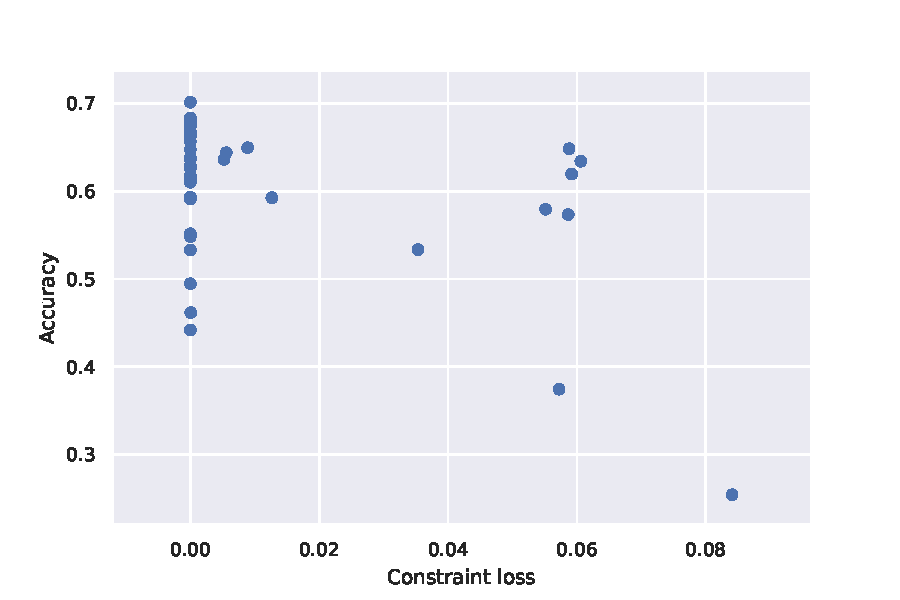
\includegraphics[width=0.5\textwidth]{constraint_loss}
      \caption{Scatter plot of constraint loss versus accuracy involving all successful tests with \cifar.}
\label{fig:constraintLoss}
\end{figure}

\begin{figure}[h]
\centering    
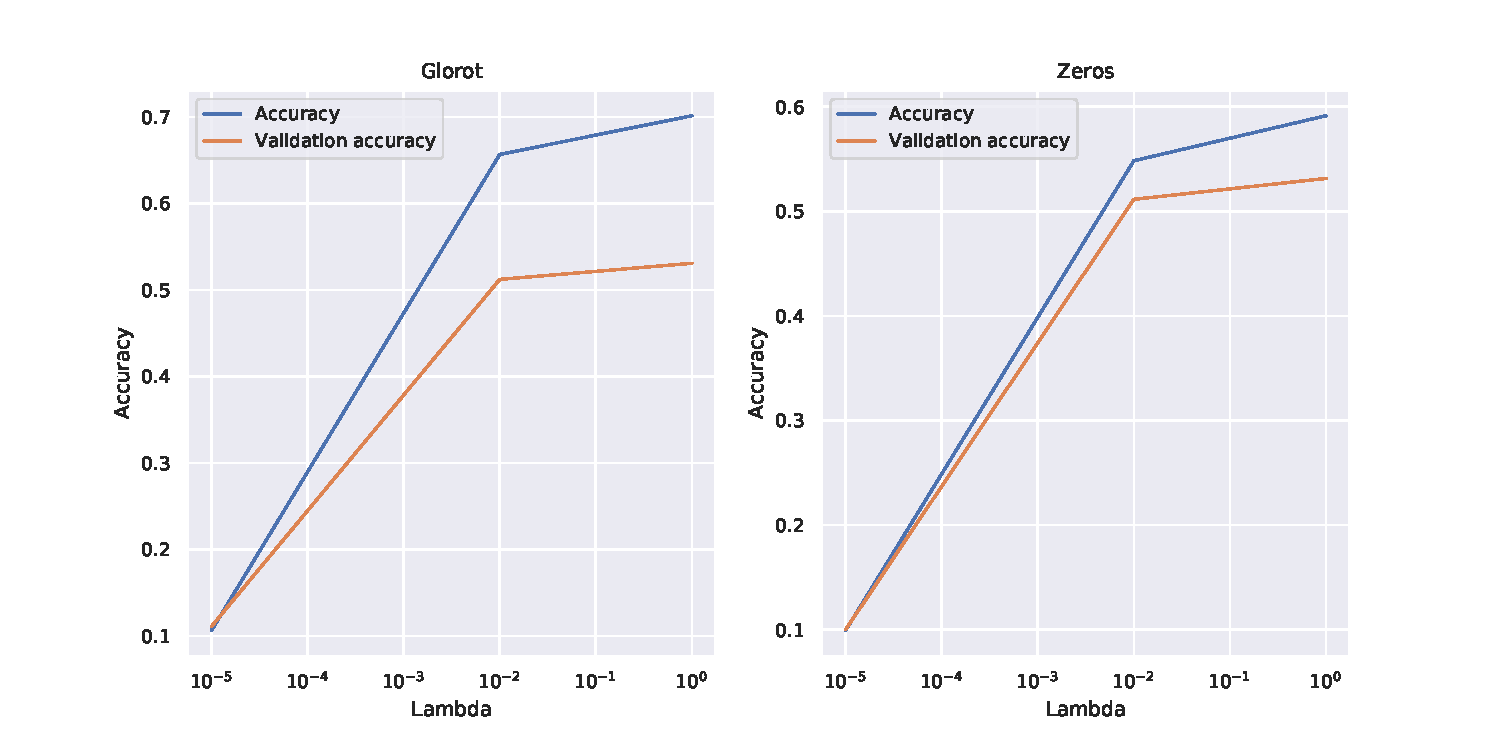
\includegraphics[width=0.5\textwidth]{lambdas}
      \caption{Accuracy versus $\lambda$. Left-hand side using Glorot initialization scheme. Right-hand side using zero intialization scheme.}
\label{fig:lambdas}
\end{figure}

\begin{figure*}[h]
  \begin{center}
    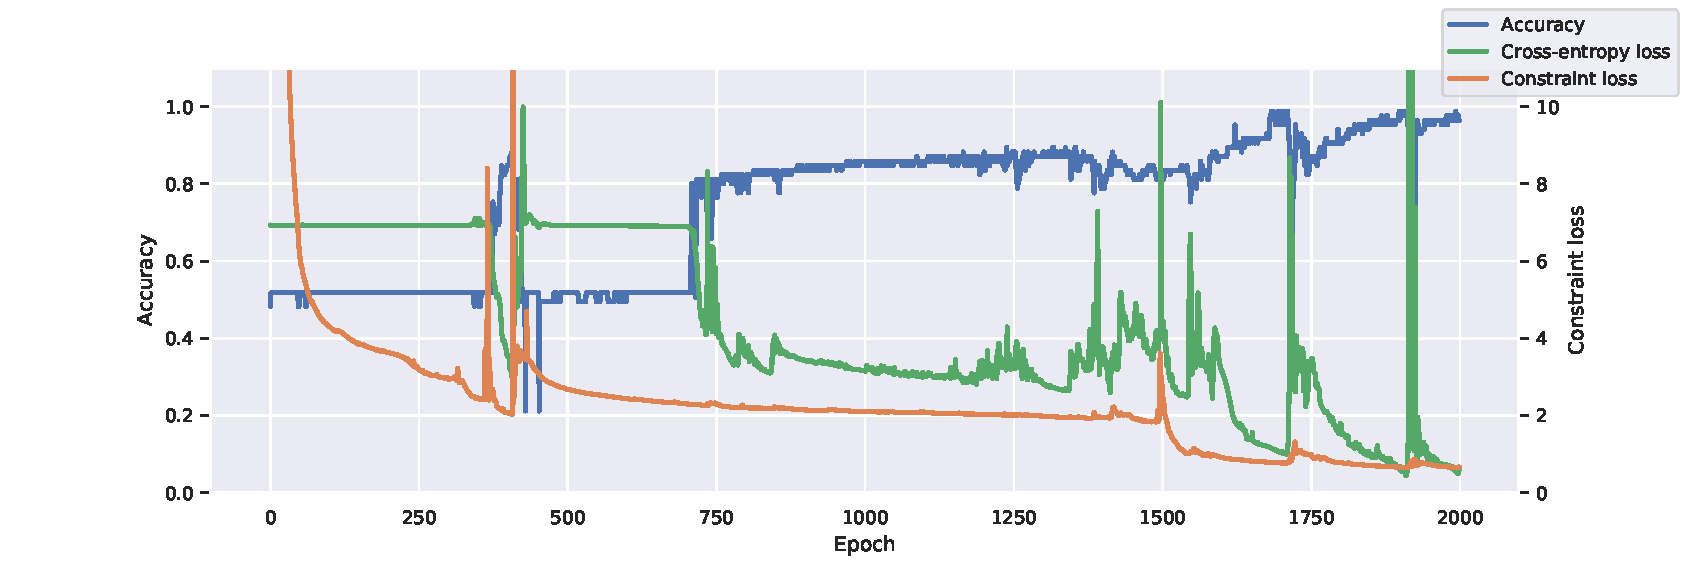
\includegraphics[width=1.0\textwidth]{peaks}
      \caption{Evolution of training throughout epochs (cross-entropy, constraint loss, and accuracy). Left-hand axis show the accuracy metric (blue line) against the cross-entropy, and constraint loss in the right axis (orange line), for each epoch of the training phase in the horizontal axis.}
			\label{fig:peaks}
\end{center}
\end{figure*}

\begin{figure*}[h]
  \centering
		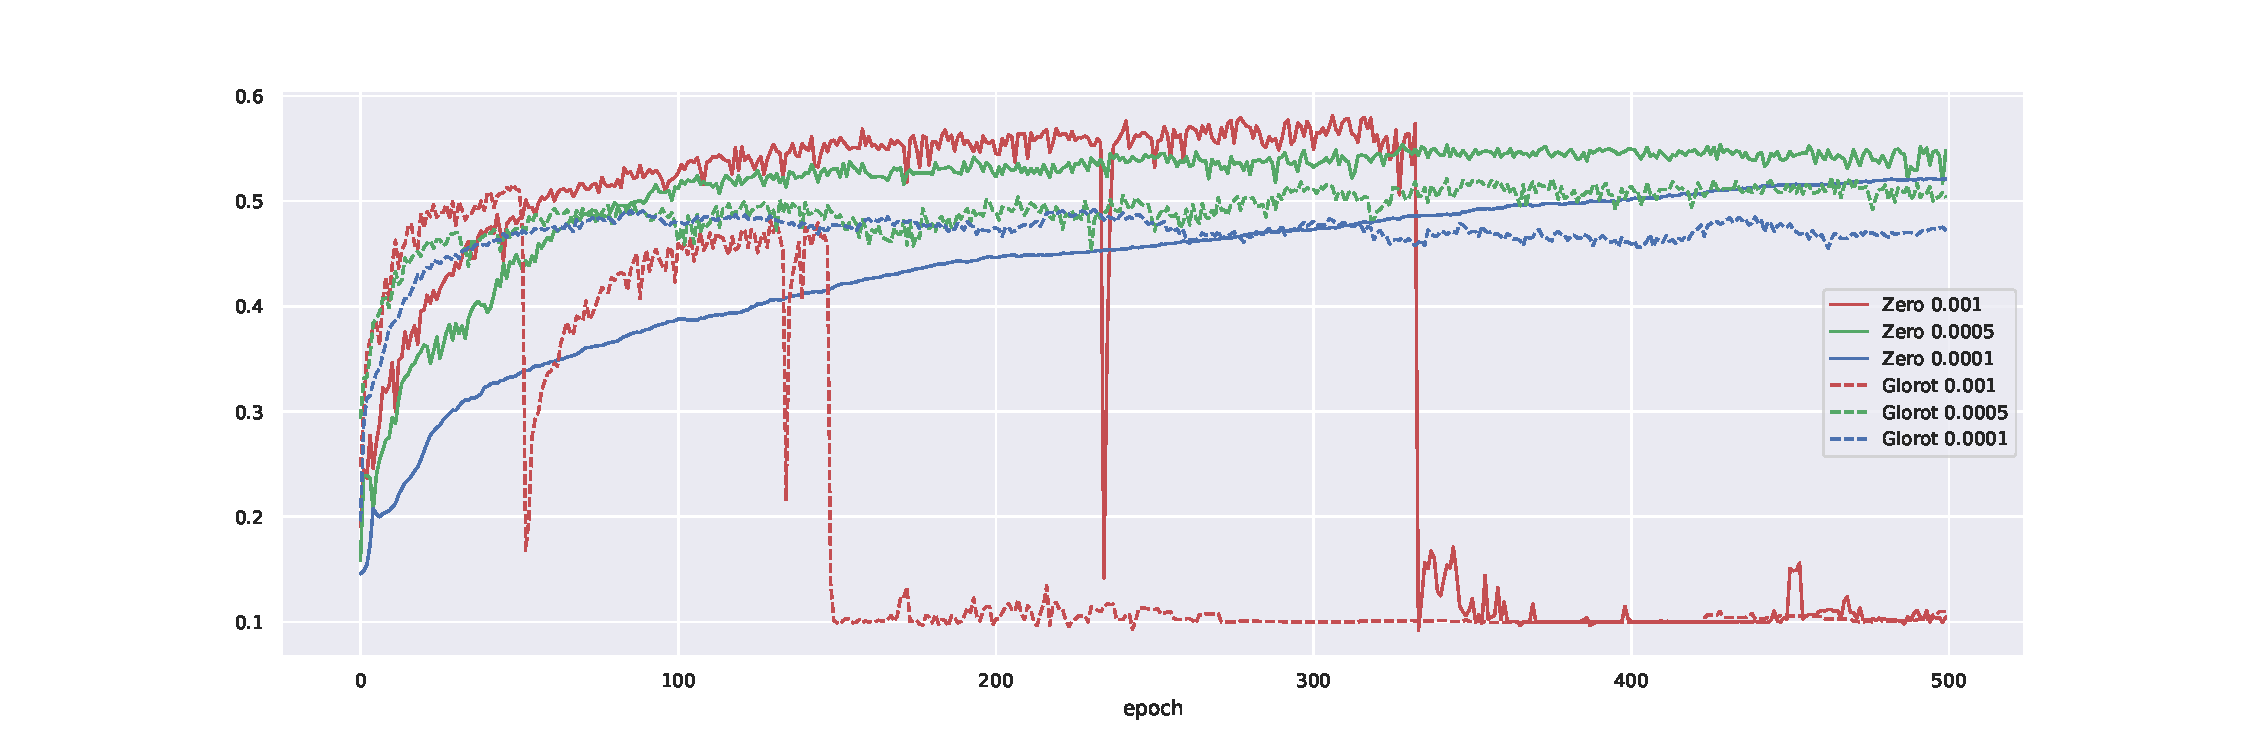
\includegraphics[width=1.0\textwidth]{zeros-vs-glorot}
      \caption{Convergence plot for the evolution of the validation accuracy during the training phase. Solid lines stand for Zero initialization, dashed stand for Glorot initialization. The colors encode the different learning rates $\gamma$ used, red for $0.001$, green for $0.0005$ and blue for $0.0001$.}
\label{fig:zeroConvergence}
\end{figure*}

\begin{figure}[h!]
\centering
    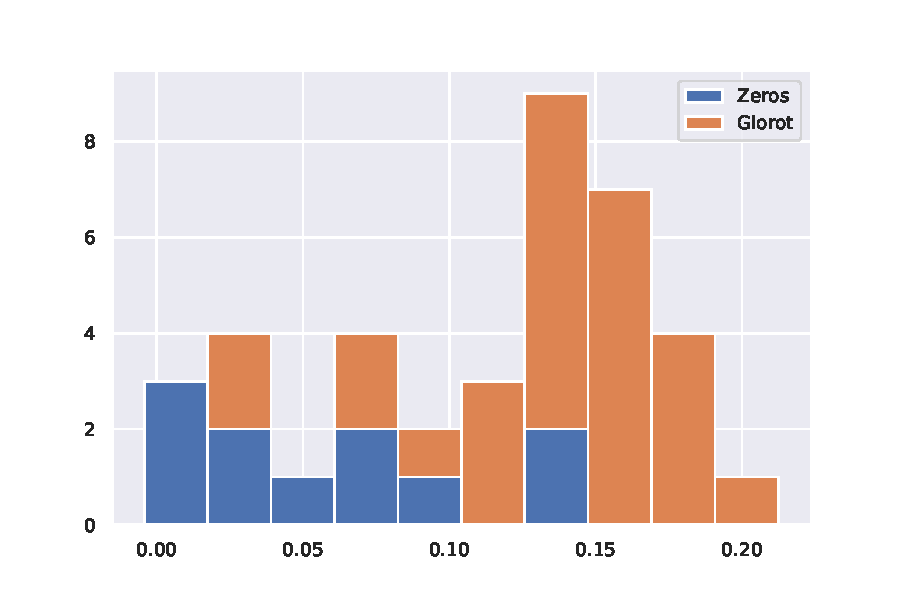
\includegraphics[width=0.5\textwidth]{zeros-vs-glorot-val-difference}
      \caption{Histogram of gaps between train and validation accuracy, for Zero and Glorot initialization over all successful runs of \cifar.}
		\label{fig:ZeroVsGlorotDifference}


\end{figure}

\begin{figure} 
    \centering
  \subfloat[Glorot weights\label{fig:glorotWeights}]{%
       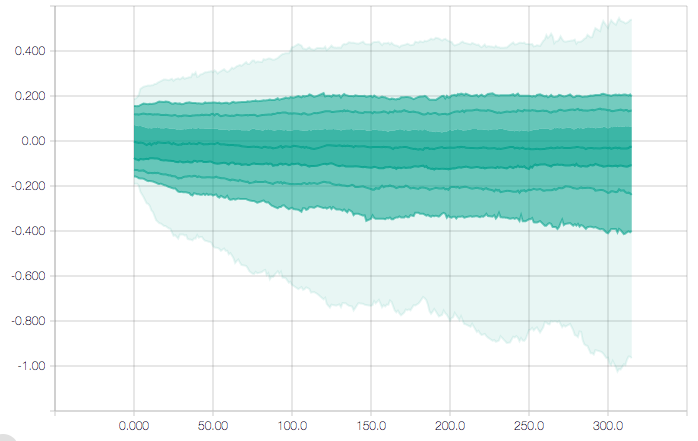
\includegraphics[width=0.45\linewidth]{glorot-kernel.png}}
    \hfill
  \subfloat[Zeros weights\label{fig:zerosWeights}]{%
        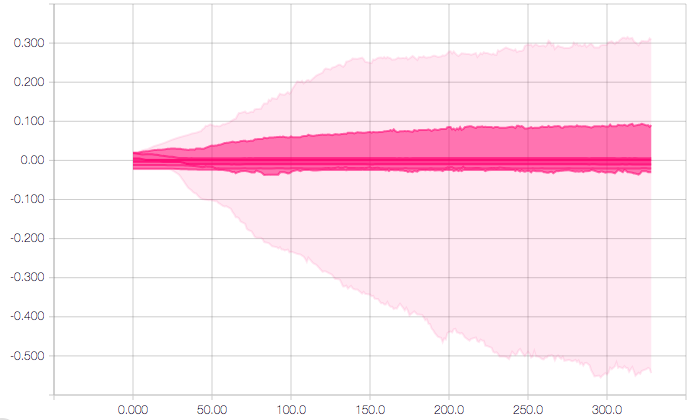
\includegraphics[width=0.45\linewidth]{zeros-kernel.png}}
    \\
  \subfloat[Glorot weight gradient\label{fig:glorotWeightGradient}]{%
        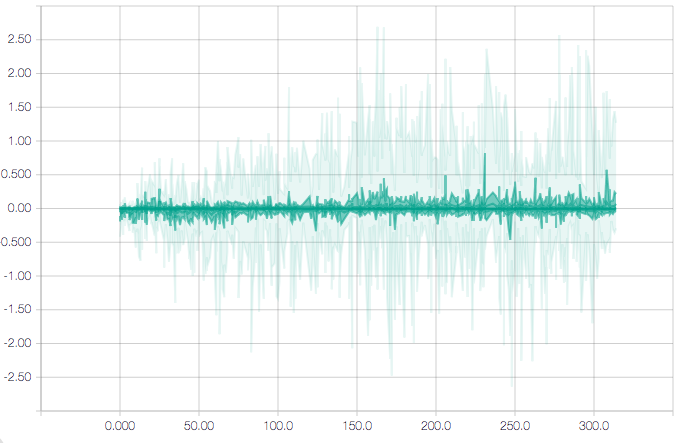
\includegraphics[width=0.45\linewidth]{glorot-kernel-grad.png}}
    \hfill
  \subfloat[Zeros weight gradient\label{fig:zerosWeightGradient}]{%
        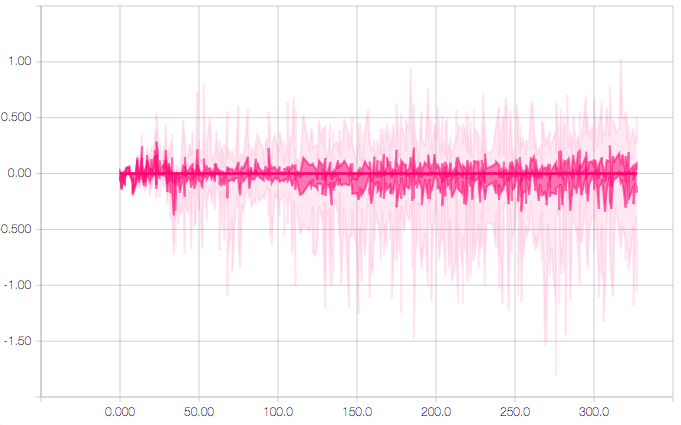
\includegraphics[width=0.45\linewidth]{zeros-kernel-grad.png}}
        
   \subfloat[Glorot bias\label{fig:glorotBias}]{%
       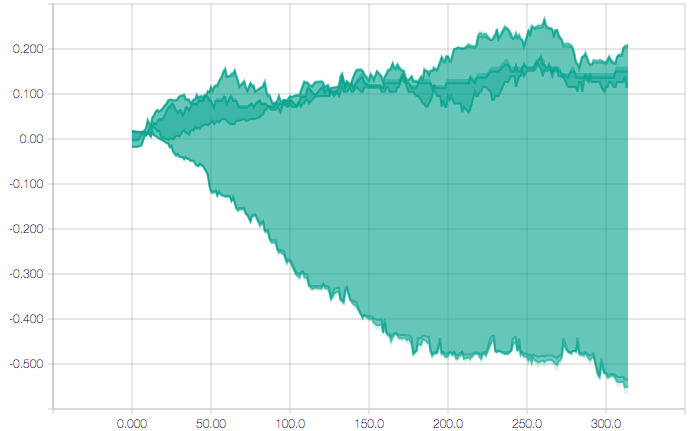
\includegraphics[width=0.45\linewidth]{glorot-bias.png}}
    \hfill
  \subfloat[Zeros bias\label{fig:zerosBias}]{%
        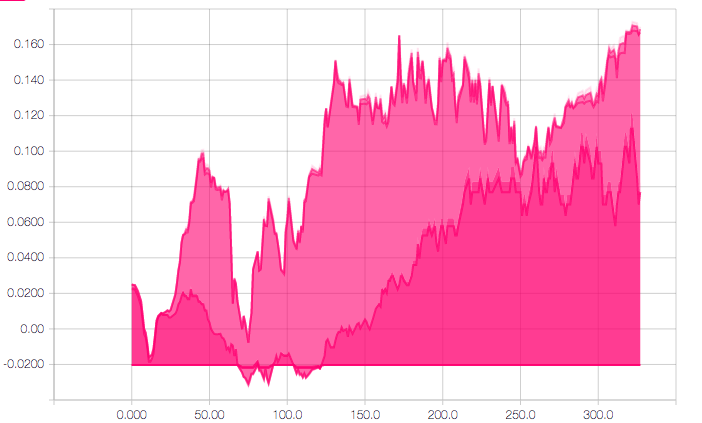
\includegraphics[width=0.45\linewidth]{zeros-bias.png}}
    \\
  \subfloat[Glorot output\label{fig:glorotOutput}]{%
        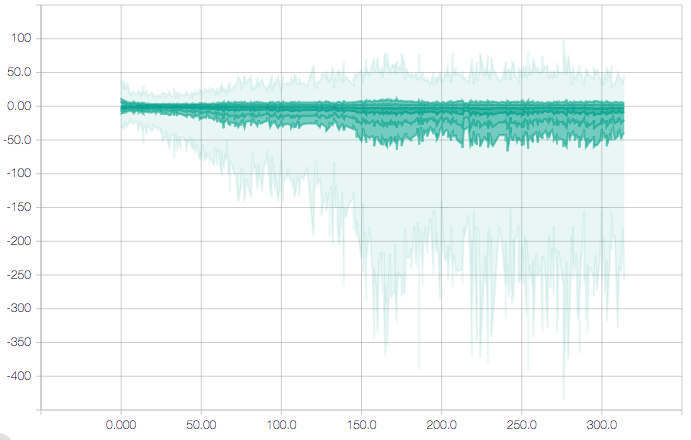
\includegraphics[width=0.45\linewidth]{glorot-out.png}}
    \hfill
  \subfloat[Zeros output\label{fig:zerosOutput}]{%
        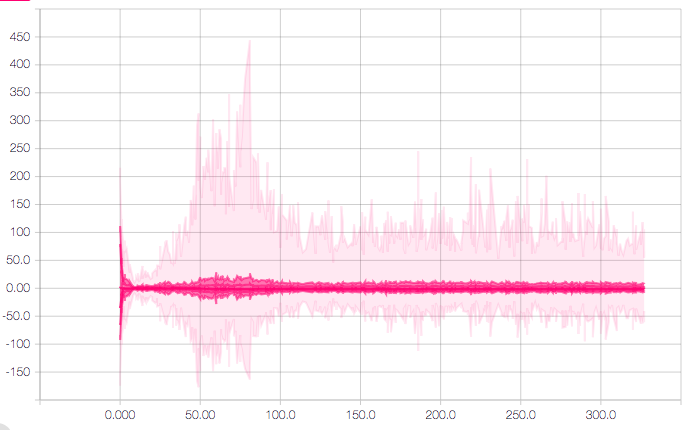
\includegraphics[width=0.45\linewidth]{zeros-out.png}}
  \caption{Histogram displaying weights, biases, gradients, and outputs from the $25$th layer constructed from a \cifar experiment, comparing zero (right-hand side in cyan) and Glorot initialization (left-hand side in magenta).}
  \label{fig:histo} 
\end{figure}
